\chapter{Experimente}
In diesem Kapitel werden Experimente mit den drei Datensätzen durchgeführt. Darüber hinaus werden verschiedene Hyperparameter getestet.

\section{Spiel-Datensatz Experimente}
\label{experimente:spiel}
Als erstes wird die Methode auf dem Spiel-Datensatz angewendet. Hierbei soll geprüft werden, ob die Methode die erwarteten
Ergebnisse liefert. Das U-Net wird für 100 Epochen mit Adam, einer Lernrate von 0.001 und der Cross Entropy Loss Function trainiert. Diese
Einstellung zeigte die besten Ergebnisse. Zeitgleich wurden Experimente mit 36 und mit 324 Bins durchgeführt, die jedoch keinen Unterschied bei den 
Ergebnissen verwiesen. Es kann davon ausgegangen werden, dass bei der niedrigen Anzahl an möglichen Farben, ein Unterschied zwischen 36 und 324 Bins
nicht zu erkennen ist. Die unteren Ergebnisse wurden mit 324 Bins erstellt.

\begin{figure}[H]
  \vspace{1cm}
  \begin{subfigure}
    \centering
    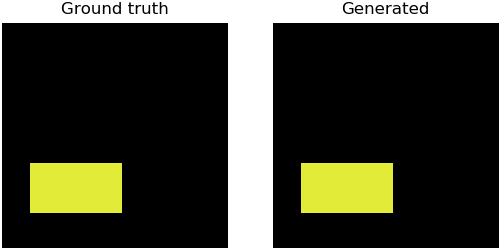
\includegraphics[width=.32\textwidth]{resources/experiments/30.png}
  \end{subfigure}
  \begin{subfigure}
    \centering
    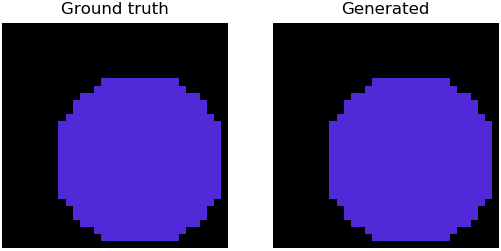
\includegraphics[width=.32\textwidth]{resources/experiments/31.png}
  \end{subfigure}
  \begin{subfigure}
    \centering
    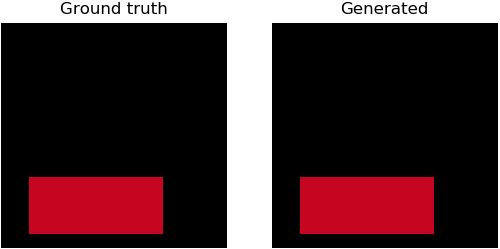
\includegraphics[width=.32\textwidth]{resources/experiments/42.png}
  \end{subfigure}
  \caption{Beispiele von sehr guten Ergebnissen aus dem Spiel-Datensatz}
  \label{image:gute-ergebnisse-toy-dataset}
\end{figure}

Bei den oberen Ergebnissen wurden alle Pixel richtig klassifiziert, was bei der Größe des Datensatzes oft zu Overfitting deutet.
Die folgenden Ergebnissen zeigen dass das Modell generalisiert und nicht overfitted hat.

\begin{figure}[H]
  \vspace{1cm}
  \begin{subfigure}
    \centering
    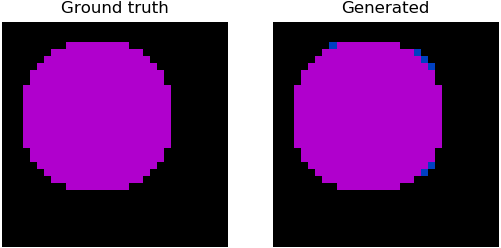
\includegraphics[width=.32\textwidth]{resources/experiments/581.png}
  \end{subfigure}
  \begin{subfigure}
    \centering
    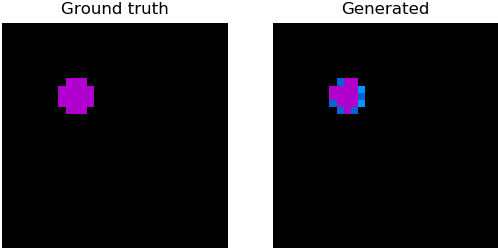
\includegraphics[width=.32\textwidth]{resources/experiments/712.png}
  \end{subfigure}
  \begin{subfigure}
    \centering
    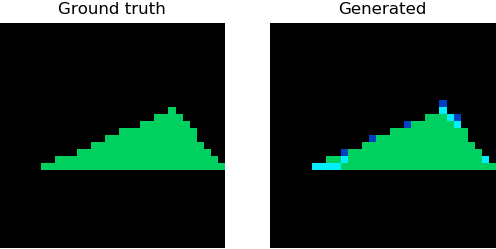
\includegraphics[width=.32\textwidth]{resources/experiments/761.png}
  \end{subfigure}
  \caption{Beispiele von generalisierten Ergebnissen}
  \label{image:nicht-gute-ergebnisse-toy-dataset}
\end{figure}

Das Model zeigte bei einigen Ergebnissen, Schwierigkeiten die Pixeln am Rand der geometrischen Formen richtig zu klassifizieren.
Dies trifft besonders auf die Kreise und Dreiecke zu, wo die Ränder nicht aus glatten Linien bestehen. Des weiteren wurden die Farben mittels
des Durchschnitts für jeden möglichen Bin, für alle Farben von jedem Trainingsbild rekonstruiert. Ein Unterschied zwischen dem Modus und dem 
Durchschnitt konnte nicht erkannt werden, da beide Werte gleich waren.
\\
Die Ergebnisse bestätigen dass das Binning und die Methode funktionieren. Anschließend wurden Experimente mit komplexeren Bildern
des Subsets von CIFAR-100 durchgeführt.

\section{CIFAR-100 Subset Experimente}\label{section:cifar-experimente}
Das Modell wurde auf 12 Klassen von CIFAR-100 über 100 Epochen mit Adam, einer Lernrate von 0.001 und der Cross Entropy Loss Function
trainiert. Diese Einstellungen stellten sich als die beste Kombination von Hyperparametern heraus, jedoch wurde das Training vor Vollendung 
von 50 Epochen unterbrochen um Overfitting zu verhindern.
% Um diesen Anstieg zu vermeiden, wurde ein Mechanismus eingeführt um die Lernrate bei einem bestimmten
% Faktor zu reduzieren wenn der Validation Loss nicht mehr sinkt oder sogar steigt. Dieser Mechanismus bietet PyTorch und wurde mit der 
% Klasse \textit{ReduceLROnPlateau} implementiert.

\begin{figure}[H]
  \centering
  \vspace{1cm}
  \begin{subfigure}
    \centering
    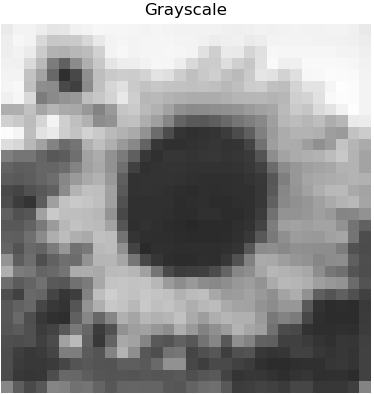
\includegraphics[width=.24\textwidth]{resources/experiments/cifar/200_grayscale.png}
  \end{subfigure}
  \begin{subfigure}
    \centering
    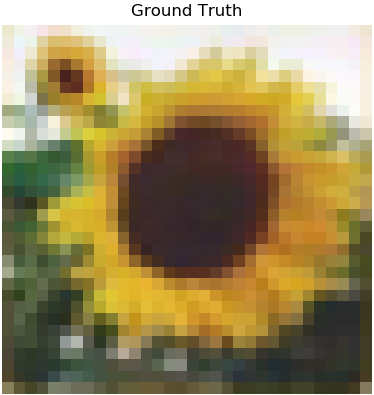
\includegraphics[width=.24\textwidth]{resources/experiments/cifar/200_original.png}
  \end{subfigure}
  \begin{subfigure}
    \centering
    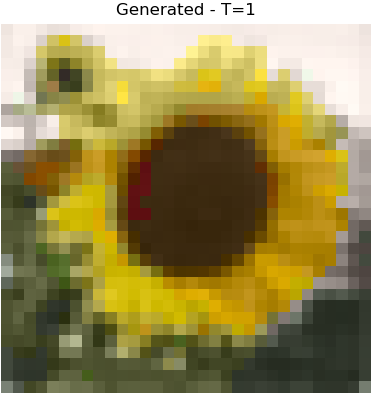
\includegraphics[width=.24\textwidth]{resources/experiments/cifar/200_t1.png}
  \end{subfigure}

  \begin{subfigure}
    \centering
    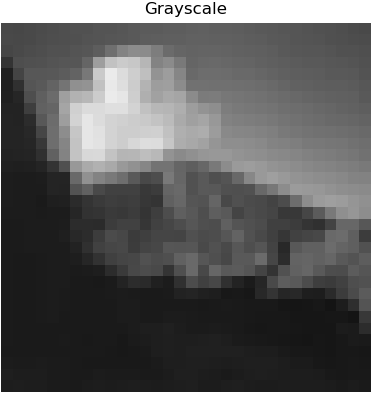
\includegraphics[width=.24\textwidth]{resources/experiments/cifar/600_grayscale.png}
  \end{subfigure}
  \begin{subfigure}
    \centering
    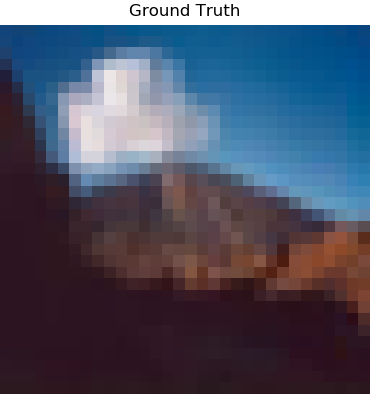
\includegraphics[width=.24\textwidth]{resources/experiments/cifar/600_original.png}
  \end{subfigure}
  \begin{subfigure}
    \centering
    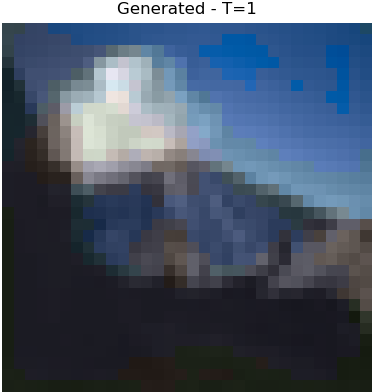
\includegraphics[width=.24\textwidth]{resources/experiments/cifar/600_t1.png}
  \end{subfigure}
  \caption{Beispiele von guten Ergebnissen aus dem Subset von CIFAR-100 mit 324 Bins. Die erste Spalte beinhaltet das Graustufenbild, die zweite Spalte
  beinhaltet das Original Bild und die letzte Spalte stellt das generierte Bild dar. Das generierte Bild wurde mit einer Temperatur von 1
  erzeugt, was bedeutet, dass die rekonstruierten Farben den Durchschnitt aus jedem Bin repräsentieren.}
  \label{image:gute-ergebnisse-cifar}
\end{figure}

Die Experimente mit diesem Datensatz haben gezeigt, dass die Anzahl der Bins bei der Auswahl an möglichen Farben, die Ergebnisse beeinträchtigen.
Eine Erhöhung der Trainingszeit zwischen 36 und 324 Bins war nicht zu erkennen.

% TODO: Change image
\begin{figure}[H]
  \centering
  \vspace{1cm}
  \begin{subfigure}
    \centering
    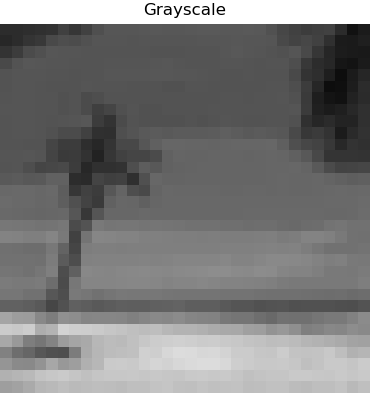
\includegraphics[width=.235\textwidth]{resources/experiments/cifar/702_grayscale.png}
  \end{subfigure}
  \begin{subfigure}
    \centering
    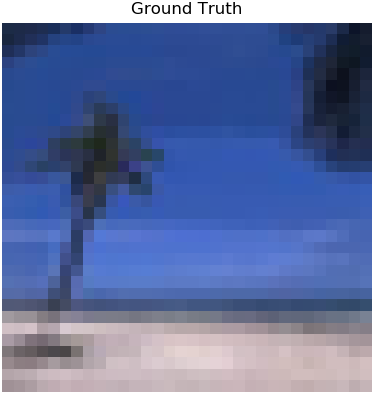
\includegraphics[width=.235\textwidth]{resources/experiments/cifar/702_original.png}
  \end{subfigure}
  \begin{subfigure}
    \centering
    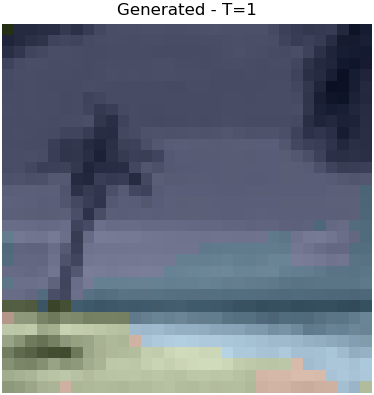
\includegraphics[width=.235\textwidth]{resources/experiments/cifar/702_36_t1.png}
  \end{subfigure}
  \begin{subfigure}
    \centering
    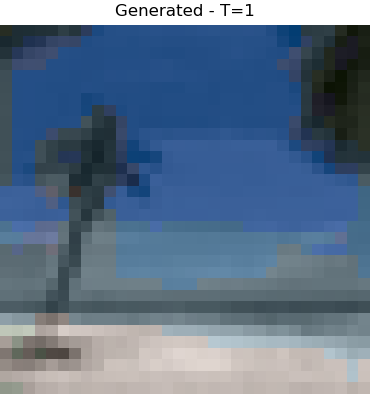
\includegraphics[width=.235\textwidth]{resources/experiments/cifar/702_t1.png}
  \end{subfigure}

  \caption{Einfluss der Anzahl der Bins auf die Ergebnisse. Das zweite Bild ist das original, das dritte Bild wurde mit 36 Bins und einem
  Temperaturwert von 1 generiert und das vierte mit 324 Bins und ebenfalls mit einem Temperaturwert von 1.}
  \label{image:gute-ergebnisse-cifar}
\end{figure}

Um das Overfitting zu verhindern wurden zahlreiche Experimente mit verschiedenen Optimierer, Aktivierungsfunktionen und Lernraten durchgeführt.
Ein Austausch von ReLU durch Tanh zeigte ein stabileres Trainingsverhalten, aber eine Verschlechterung der Validation Loss. Leaky ReLU zeigte 
ein ähnliches Verhalten wie ReLU, aber keine Verbesserung der Ergebnissen. Die Verwendung von RMSprop anstelle von Adam zeigte eine langsamere Konvergenz Richtung Minimum.
Abschließend wurde die Anzahl der Filter in den Convolutional Layers halbiert, was eine positive Wirkung auf das Training hatte.   

\subsection{Experimente mit MSE Loss und ohne Binning}
Um die Performance der Klassifikation gegenüber der Regression zu messen, wurde ein Modell mit der MSE Loss Function trainiert. Dieses Model
wurde ebenfalls mit den gleichen Parametern wie das Klassifikationsmodell trainiert und hat vergleichbare Ergebnisse erreicht. Einige Ergebnisse
zeigten blasse stellen im Vergleich zu dem Klassifikationsmodell, der leuchtende Farben an den gleichen Stellen gezeigt hat.

\begin{figure}[H]
  \centering
  \vspace{1cm}
  \begin{subfigure}
    \centering
    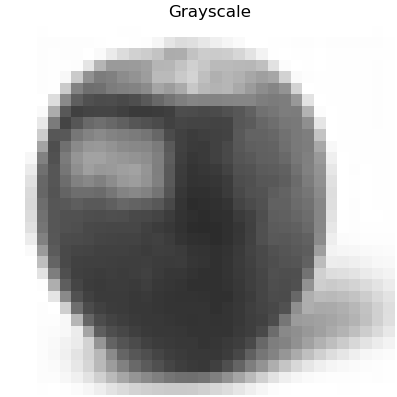
\includegraphics[width=.235\textwidth]{resources/experiments/cifar/311_grayscale.png}
  \end{subfigure}
  \begin{subfigure}
    \centering
    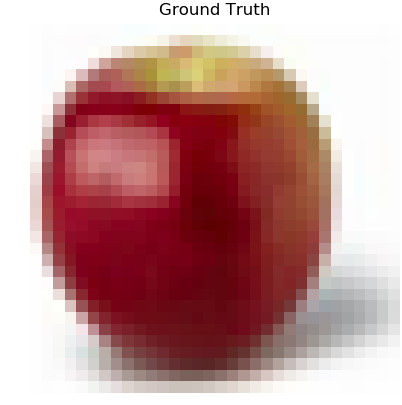
\includegraphics[width=.235\textwidth]{resources/experiments/cifar/311_original.png}
  \end{subfigure}
  \begin{subfigure}
    \centering
    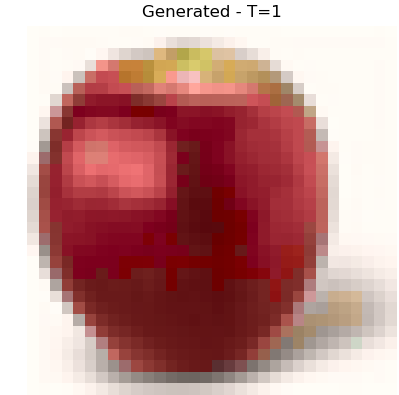
\includegraphics[width=.235\textwidth]{resources/experiments/cifar/311_t1.png}
  \end{subfigure}
  \begin{subfigure}
    \centering
    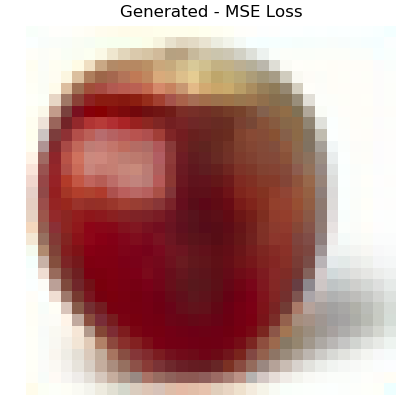
\includegraphics[width=.235\textwidth]{resources/experiments/cifar/311_regression.png}
  \end{subfigure}

  \caption{Vergleich von Klassifikation mit Binning gegenüber Regression. Das zweite Bild wurde mit 324 Bins und dem Cross Entropy Loss generiert.
  Das dritte Bild wurde ohne Binning und mit einem MSE Loss generiert.}
  \label{image:mse-ergebnisse-cifar}
\end{figure}

\section{Landscape Datensatz Experimente}
Dieser Datensatz wurde anhand der Hyperparameter Optimierung von den CIFAR-100 Subset trainiert. Es wurde das größere Model für $128 \times 128$
Input Bilder angewendet. Das Model wurde ebenfalls für 36 und 324 Bins, mit dem Adam Optimizer, eine Lernrate von 0.001 und die Cross Entropy 
Loss Function für 60 Epochen trainiert. Das Model mit den besten Validation Loss wurde gespeichert um die Ergebnisse zu evaluieren. Außerdem
wurden den Einfluss der Temperaturwert und der Anzahl der Bins auf die Ergebnisse gemessen.
\\
\\
Das Model tendierte ebenfalls bei diesem Datensatz zum Overfitting. Um das zu verhindern wurden die gleiche Techniken wie bei CIFAR-100
angewendet, was keine bessere Ergebnisse geliefert hat. Eine Halbierung der Anzahl der Filter bei den Convolutional Layers erwiesen eine Verschlechterung
des Validation Loss und half nicht bei Overfitting. Eine Änderung der Optimierer zu RMSprop und die Ersetzung von ReLU durch Tanh zeigten
einen stabileren Training aber keine Verbesserung der Validation Loss. Das Endgültige Model wurde trainiert bis der Validation Loss wieder stieg.

\begin{figure}[H]
  \centering
  \vspace{1cm}
  \begin{subfigure}
    \centering
    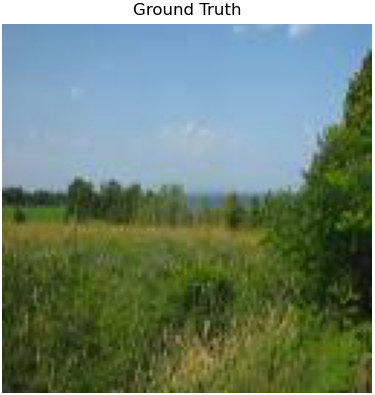
\includegraphics[width=.235\textwidth]{resources/experiments/landscape/324_bins/028/028_original.png}
  \end{subfigure}
  \begin{subfigure}
    \centering
    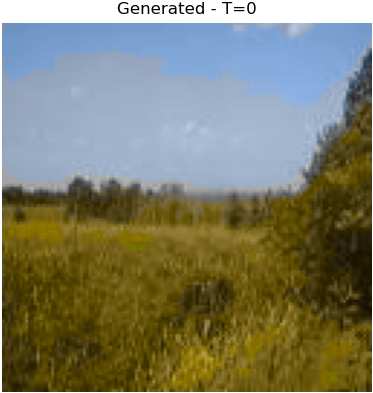
\includegraphics[width=.235\textwidth]{resources/experiments/landscape/324_bins/028/028_t0.png}
  \end{subfigure}
  \begin{subfigure}
    \centering
    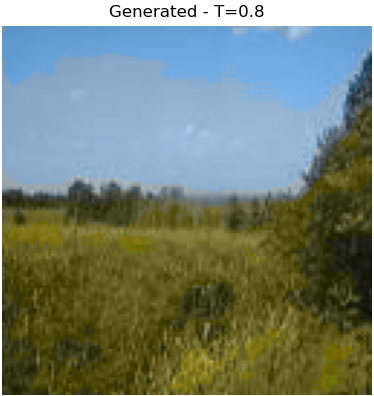
\includegraphics[width=.235\textwidth]{resources/experiments/landscape/324_bins/028/028_t08.png}
  \end{subfigure}
  \begin{subfigure}
    \centering
    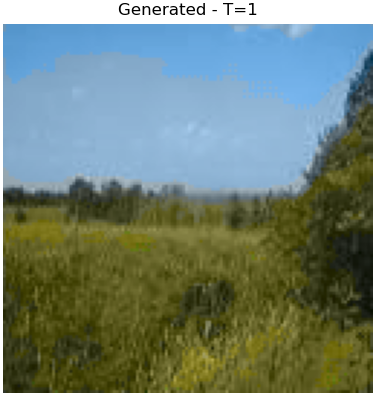
\includegraphics[width=.235\textwidth]{resources/experiments/landscape/324_bins/028/028_t1.png}
  \end{subfigure}

  \begin{subfigure}
    \centering
    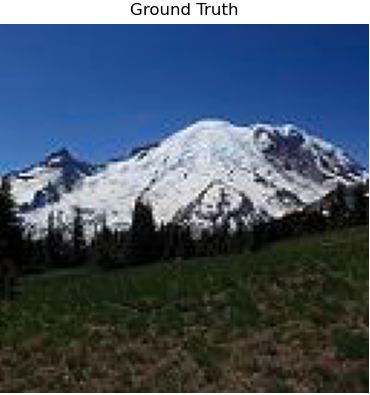
\includegraphics[width=.235\textwidth]{resources/experiments/landscape/324_bins/736/736_original.png}
  \end{subfigure}
  \begin{subfigure}
    \centering
    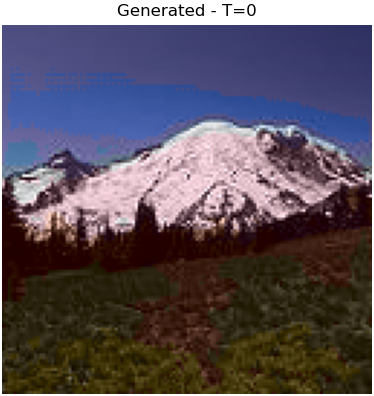
\includegraphics[width=.235\textwidth]{resources/experiments/landscape/324_bins/736/736_t0.png}
  \end{subfigure}
  \begin{subfigure}
    \centering
    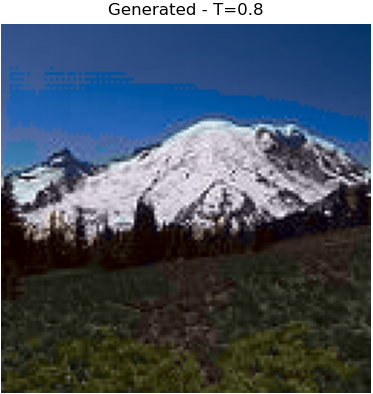
\includegraphics[width=.235\textwidth]{resources/experiments/landscape/324_bins/736/736_t08.png}
  \end{subfigure}
  \begin{subfigure}
    \centering
    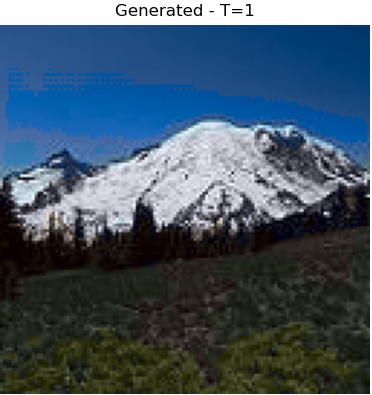
\includegraphics[width=.235\textwidth]{resources/experiments/landscape/324_bins/736/736_t1.png}
  \end{subfigure}

  \caption{Ergebnisse mit 324 Bins. Die erste Spalte zeigt das Originale Bild, die zweite zeigt das generierte Bild mit einer Temperatur von 0,
  die dritte Spalte zeigt das generierte Bild mit einer Temperatur von 0.8 und die vierte Spalte zeigt das generierte Bild mit einer Temperatur 
  von 1}
  \label{image:gute-ergebnisse-own}
\end{figure}

Nach der Auswertung der Experimente würden 324 Bins und ein Temperaturwert von 0.8 bis 1 bevorzugt um die bestmöglichen Ergebnissen zu bekommen.

\begin{figure}[H]
  \centering
  \vspace{1cm}
  \begin{subfigure}
    \centering
    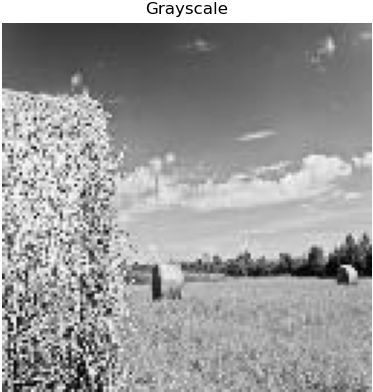
\includegraphics[width=.235\textwidth]{resources/experiments/landscape/324_bins/342/342_grayscale.png}
  \end{subfigure}
  \begin{subfigure}
    \centering
    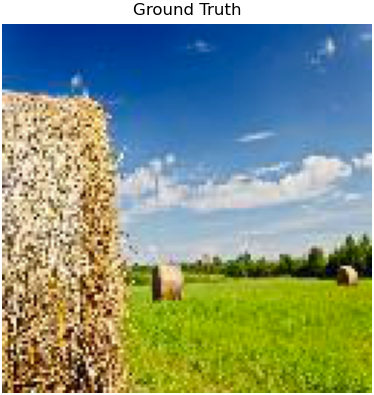
\includegraphics[width=.235\textwidth]{resources/experiments/landscape/324_bins/342/342_original.png}
  \end{subfigure}
  \begin{subfigure}
    \centering
    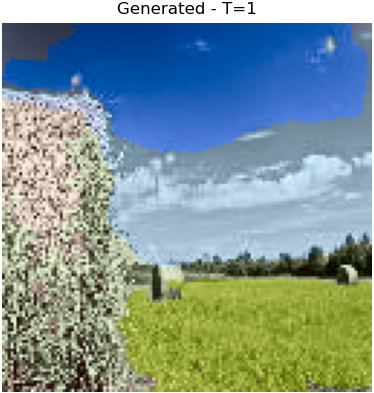
\includegraphics[width=.235\textwidth]{resources/experiments/landscape/36_bins/342/342_t1.png}
  \end{subfigure}
  \begin{subfigure}
    \centering
    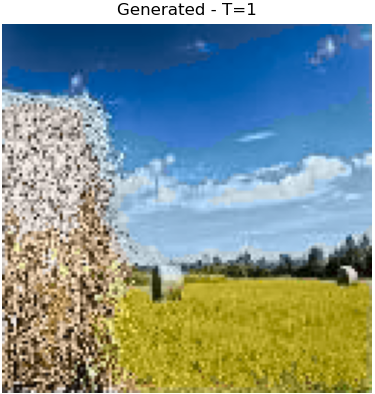
\includegraphics[width=.235\textwidth]{resources/experiments/landscape/324_bins/342/342_t1.png}
  \end{subfigure}

  \caption{Ergebnisse mit 36 und 324 Bins. Die erste Spalte zeigt das Graustufenbild, die zweite zeigt das originale Bild,
  die dritte Spalte zeigt das mit 36 Bins generierte Bild mit einer Temperatur von 1 und die vierte Spalte zeigt das mit 324 Bins generierte 
  Bild mit einer Temperatur von 1}
  \label{image:bins-ergebnisse-own}
\end{figure}